\documentclass[11pt]{article}
\usepackage[margin=1in]{geometry}
\usepackage{amsmath,amssymb,amsthm}
\usepackage{graphicx}
\usepackage{booktabs}
\usepackage{hyperref}
\usepackage{cleveref}
\usepackage{natbib}
\usepackage{float}
\newtheorem{theorem}{Theorem}
\newtheorem{proposition}{Proposition}
\newtheorem{lemma}{Lemma}
\newtheorem{corollary}{Corollary}
\theoremstyle{definition}
\newtheorem{definition}{Definition}
\title{\textbf{Forecasting Hourly Air Pollution in Beijing Using Weather Data}}
\author{Cardin Tran, Jimmy Rubio-Gonalez, Isaac Humphries, Vamsi Marrapu,\\ Abdul Mutaal, Nhi Tran, Renee Vo, David Zhong}
\date{}
\begin{document}
\maketitle
\begin{abstract}
Fine particulate matter (PM2.5) is an important indicator of air pollution. This study examines how well weather and calendar variables explain hourly PM2.5 concentrations in Beijing using the UCI Beijing PM2.5 dataset from 2010--2014. After removing 2,067 observations without a PM2.5 measurement, 41,757 labeled observations remain. We compare a mean baseline, ordinary least-squares Linear Regression, Ridge Regression, and Random Forest Regression. Models are initially assessed on 2013 after training on 2010--2012, then refitted on 2010--2013 and evaluated on a held-out 2014 test set. Random Forest achieves the best test performance (MAE 48.073 $\mu$g/m$^3$, RMSE 71.397 $\mu$g/m$^3$, $R^2=0.417$), outperforming the linear models and baseline. The results suggest that nonlinear relationships are useful for estimating PM2.5 from meteorological and calendar conditions, although substantial unexplained variation remains. Because the inputs describe the same hour as the target, this experiment evaluates contemporaneous estimation rather than an operational future-hour forecast.
\end{abstract}
\noindent\textbf{Keywords:} Air Pollution, PM2.5, Machine Learning, Regression, Random Forest, Weather Data, Forecasting

\section{Introduction}
Airborne fine particulate matter, commonly described as PM2.5, consists of particles with aerodynamic diameters of approximately 2.5 micrometers or smaller. High concentrations are a public-health concern, making it useful to understand the relationship between pollution levels and routinely recorded environmental conditions. Meteorological variables may be associated with the accumulation or dispersion of pollutants, but these relationships can be nonlinear and affected by unobserved emission sources.

Our research question is: \emph{How accurately can common regression methods estimate hourly PM2.5 concentrations in Beijing from weather observations and calendar information?} We compare three regression algorithms against a simple mean predictor using the same features and chronological evaluation periods. Our original proposal used the term ``forecasting.'' In the completed implementation, the weather features and PM2.5 measurement belong to the same hour. We therefore use ``estimation'' for the actual prediction task and reserve ``forecasting'' for future work with a defined prediction horizon.

\section{Related Work}
The UCI Beijing PM2.5 dataset provides hourly pollution and weather measurements for a five-year historical period and is intended for regression analysis \citep{uci381}. Standard linear regression offers an interpretable additive model; Ridge Regression adds an $L_2$ penalty to shrink coefficients; and Random Forest Regression combines multiple decision trees to capture nonlinear relationships and interactions \citep{sklearnlinear,sklearnridge,sklearnforest}. These methods represent a useful range of complexity for a comparative undergraduate machine learning study. Rather than claiming an exhaustive review of air-pollution prediction research, this report focuses on the methods implemented and the results measured in our experiment.

\section{Preliminaries}
Let $y_i$ denote the measured PM2.5 concentration and $\hat y_i$ the model's estimate, both in $\mu$g/m$^3$. The baseline predicts the mean PM2.5 concentration in the training set. Linear Regression estimates $\hat y=\beta_0+\sum_j\beta_j x_j$, while Ridge minimizes squared prediction error with an additional penalty proportional to $\alpha\sum_j\beta_j^2$ (excluding the intercept). Random Forest averages predictions from an ensemble of regression trees.

For $n$ observations, evaluation uses
\begin{align}
\mathrm{MAE} &= \frac{1}{n}\sum_{i=1}^{n}|y_i-\hat y_i|,\\
\mathrm{RMSE} &= \sqrt{\frac{1}{n}\sum_{i=1}^{n}(y_i-\hat y_i)^2},\\
R^2 &= 1-\frac{\sum_{i=1}^{n}(y_i-\hat y_i)^2}{\sum_{i=1}^{n}(y_i-\bar y)^2},
\end{align}
where $\bar y$ is the mean observed target in the evaluated split. Lower MAE and RMSE indicate smaller errors; higher $R^2$ indicates better explanatory performance relative to predicting the evaluated split's mean. RMSE penalizes large errors more heavily than MAE.

\section{Methodology}
\subsection{Dataset and cleaning}
We use the original \texttt{PRSA\_data\_2010.1.1-2014.12.31.csv} from the UCI Beijing PM2.5 dataset \citep{uci381}. It contains 43,824 hourly rows and 13 columns, including the target \texttt{pm2.5}, date/time fields, and meteorological variables. The observed PM2.5 values span 0 to 994 $\mu$g/m$^3$; among nonmissing targets, the median is 72 $\mu$g/m$^3$.

There are 2,067 missing PM2.5 targets, which are removed rather than imputed because the target is required for supervised evaluation. This leaves 41,757 observations. The original file has no missing entries in the selected meteorological input columns, although the preprocessing pipeline is configured to impute future missing numeric or categorical features if encountered. The code parses and sorts timestamps, checks that timestamps are unique, and constructs a categorical season from month.

\subsection{Features and transformations}
The numeric features are temperature (\texttt{TEMP}), dew point (\texttt{DEWP}), pressure (\texttt{PRES}), cumulative wind speed (\texttt{Iws}), accumulated snow hours (\texttt{Is}), accumulated rain hours (\texttt{Ir}), hour, and month. The categorical features are combined wind direction (\texttt{cbwd}) and season. Numeric inputs pass through median imputation and standard scaling; categorical inputs pass through most-frequent imputation and one-hot encoding. These transformations are fit within a scikit-learn pipeline using only the corresponding training split, avoiding leakage of validation or test information into fitted preprocessing parameters.

The dataset's row index and PM2.5 target are not used as input features. Calendar year is used to define the chronological split rather than supplied to the regression models.

\subsection{Models}
The baseline is \texttt{DummyRegressor(strategy="mean")}. Linear Regression uses the default ordinary least-squares estimator. Ridge uses $\alpha=1.0$. Random Forest uses 100 trees, a minimum of two samples per leaf, and random seed 42. These settings are fixed in the submitted implementation; no hyperparameter search is performed. All four models use the same feature set and comparable preprocessing pipelines.

\section{Experimental Setup}
We use a chronological development and test protocol to avoid randomly mixing earlier and later observations. The initial training period is 2010--2012 (24,418 labeled observations), and 2013 is the validation period (8,678 observations). After comparing performance on 2013, the models are retrained on all available labeled data from 2010--2013 (33,096 observations) and evaluated once on 2014 (8,661 observations). This yields a 41,757-row labeled dataset in total.

All experiments use Python, pandas, NumPy, scikit-learn, matplotlib, and seaborn. The submitted repository provides \texttt{main.py} as the entry point and separates loading, preprocessing, training, and evaluation into modules in \texttt{src/}. Running \texttt{python main.py} saves a CSV of validation and test metrics and three figures. The reported numbers below come from the supplied execution output and \texttt{results/model\_comparison.csv}, not from hypothetical runs.

\section{Results}
\begin{table}[H]
\centering
\caption{Validation performance on 2013 ($n=8{,}678$). MAE and RMSE are in $\mu$g/m$^3$.}
\label{tab:validation}
\begin{tabular}{lrrr}\toprule
Model & MAE & RMSE & $R^2$ \\\midrule
Mean baseline & 70.923 & 98.142 & -0.002 \\
Linear Regression & 58.141 & 82.224 & 0.297 \\
Ridge Regression & 58.139 & 82.225 & 0.297 \\
Random Forest & \textbf{48.385} & \textbf{74.493} & \textbf{0.423} \\\bottomrule
\end{tabular}
\end{table}

\begin{table}[H]
\centering
\caption{Held-out test performance on 2014 ($n=8{,}661$). MAE and RMSE are in $\mu$g/m$^3$.}
\label{tab:test}
\begin{tabular}{lrrr}\toprule
Model & MAE & RMSE & $R^2$ \\\midrule
Mean baseline & 69.161 & 93.533 & -0.000 \\
Linear Regression & 55.680 & 79.057 & 0.285 \\
Ridge Regression & 55.679 & 79.057 & 0.285 \\
Random Forest & \textbf{48.073} & \textbf{71.397} & \textbf{0.417} \\\bottomrule
\end{tabular}
\end{table}

Random Forest has the lowest test MAE and RMSE and the highest $R^2$. Compared with the mean baseline, its test MAE is approximately 30.5\% lower and RMSE approximately 23.7\% lower. Its RMSE is approximately 9.7\% lower than that of Linear Regression. Linear and Ridge Regression perform almost identically with the chosen Ridge penalty. Random Forest also ranks first on the 2013 validation period, so the relative ranking is consistent across these two held-out years.

\begin{figure}[H]\centering
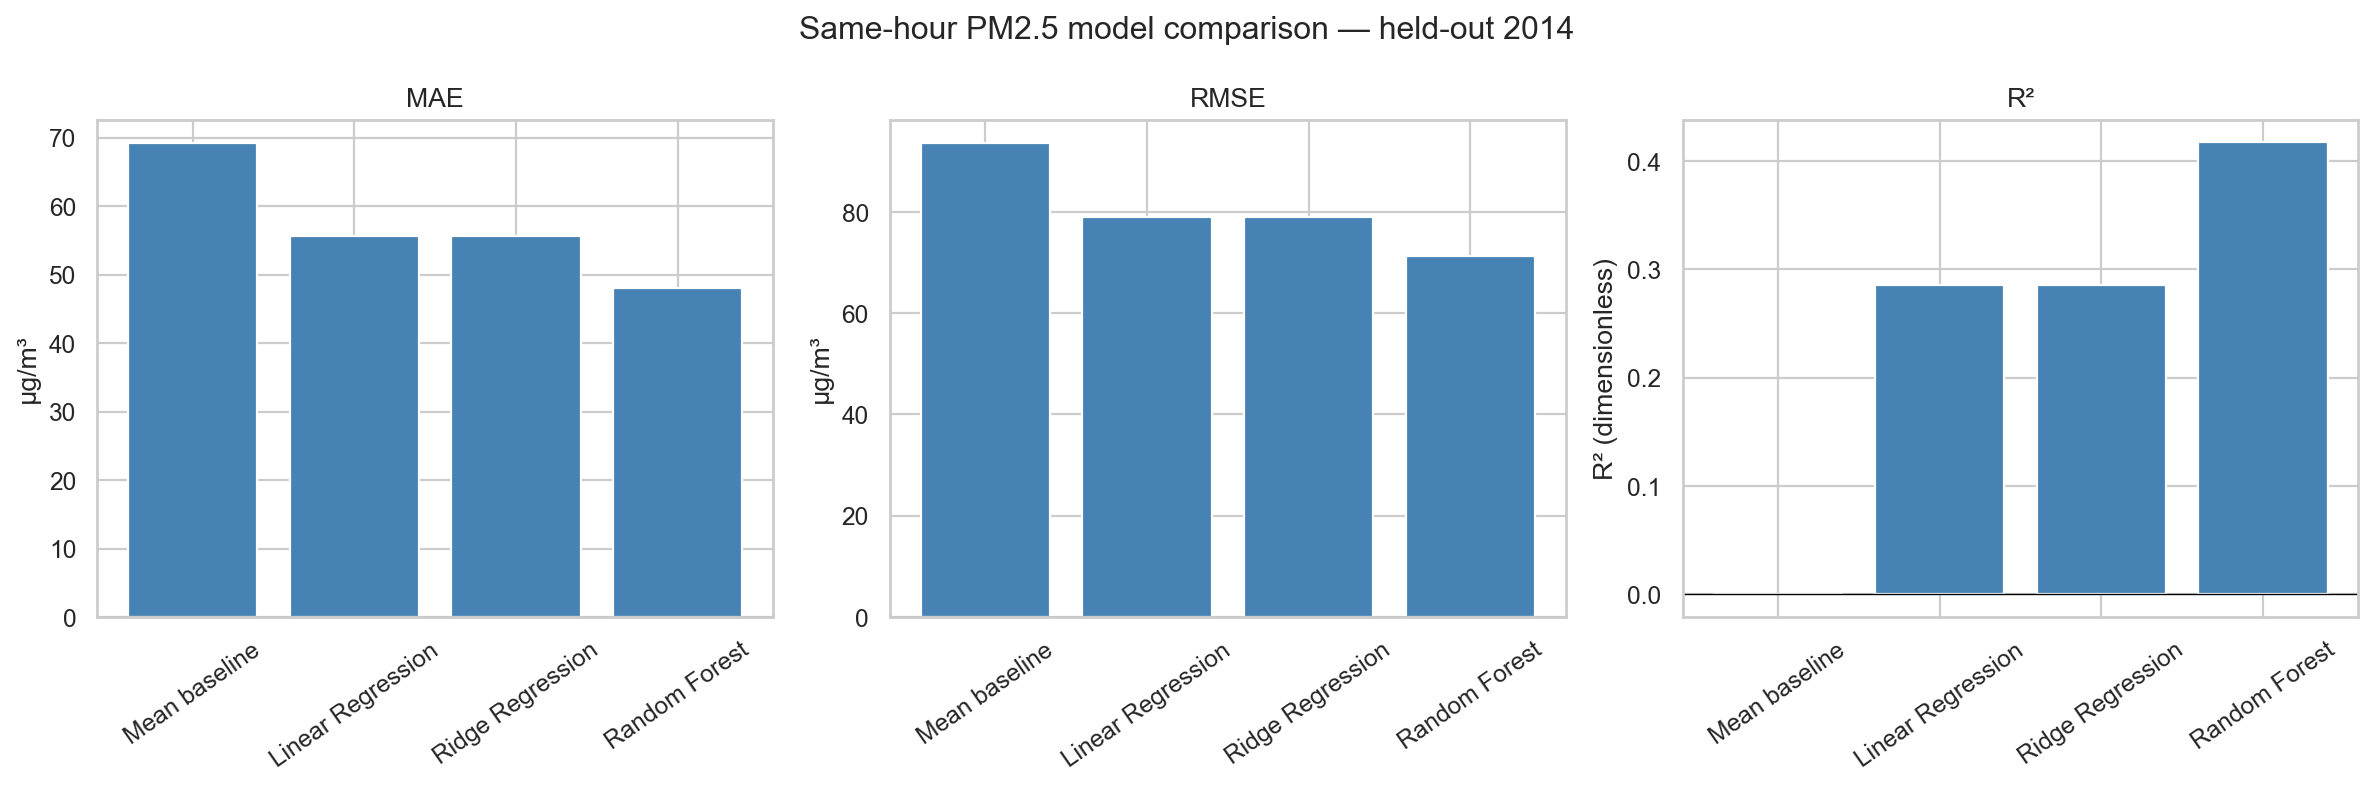
\includegraphics[width=\textwidth]{figures/model_comparison.png}
\caption{Held-out 2014 performance of the four regression approaches. The negative baseline $R^2$ is very close to zero.}\label{fig:comparison}
\end{figure}

\begin{figure}[H]\centering
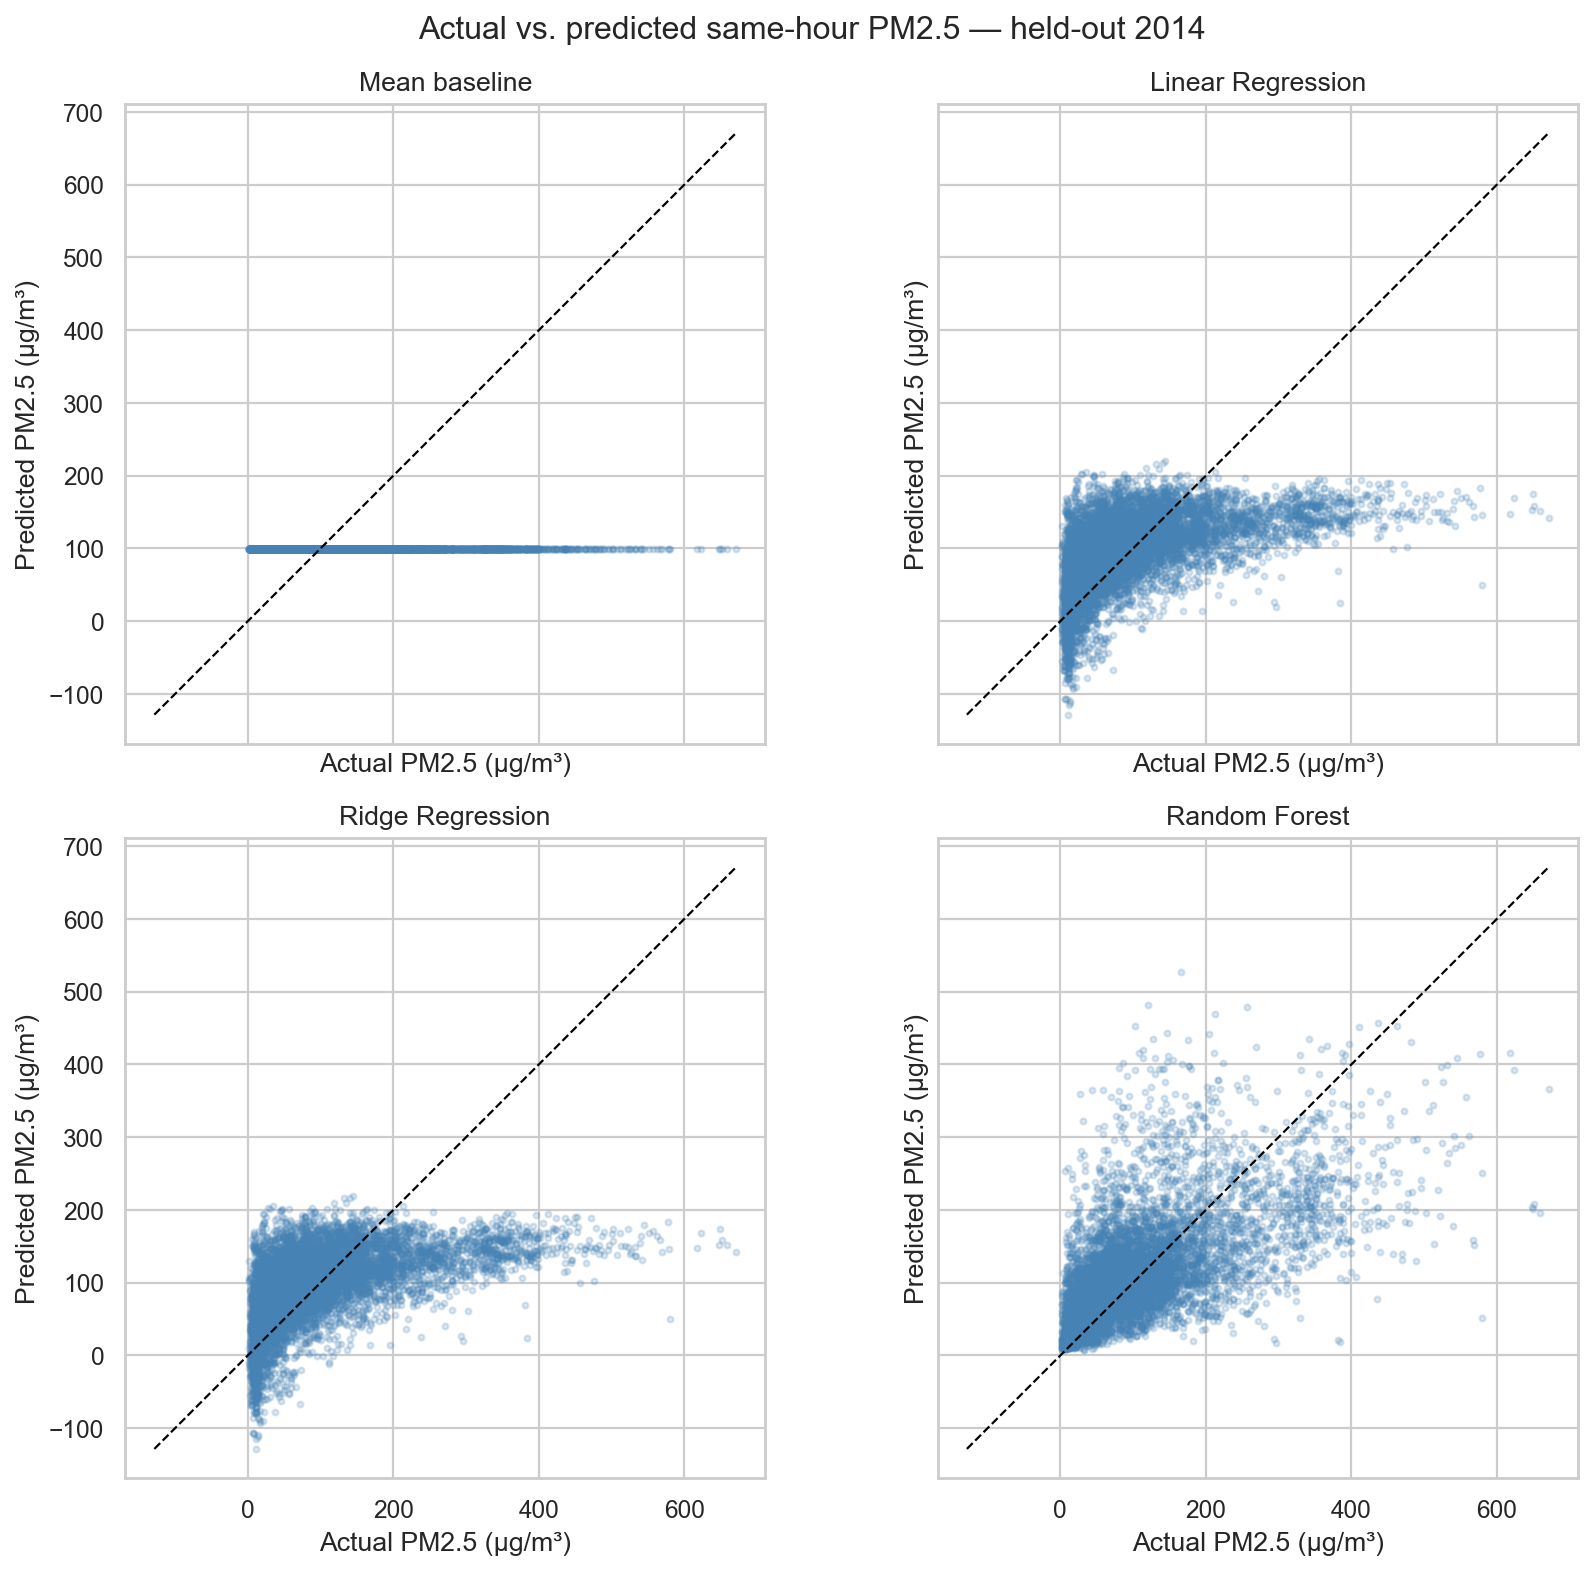
\includegraphics[width=0.83\textwidth]{figures/actual_vs_predicted.png}
\caption{Observed versus estimated PM2.5 for the 2014 test period. The dashed diagonal denotes perfect agreement.}\label{fig:predicted}
\end{figure}

\begin{figure}[H]\centering
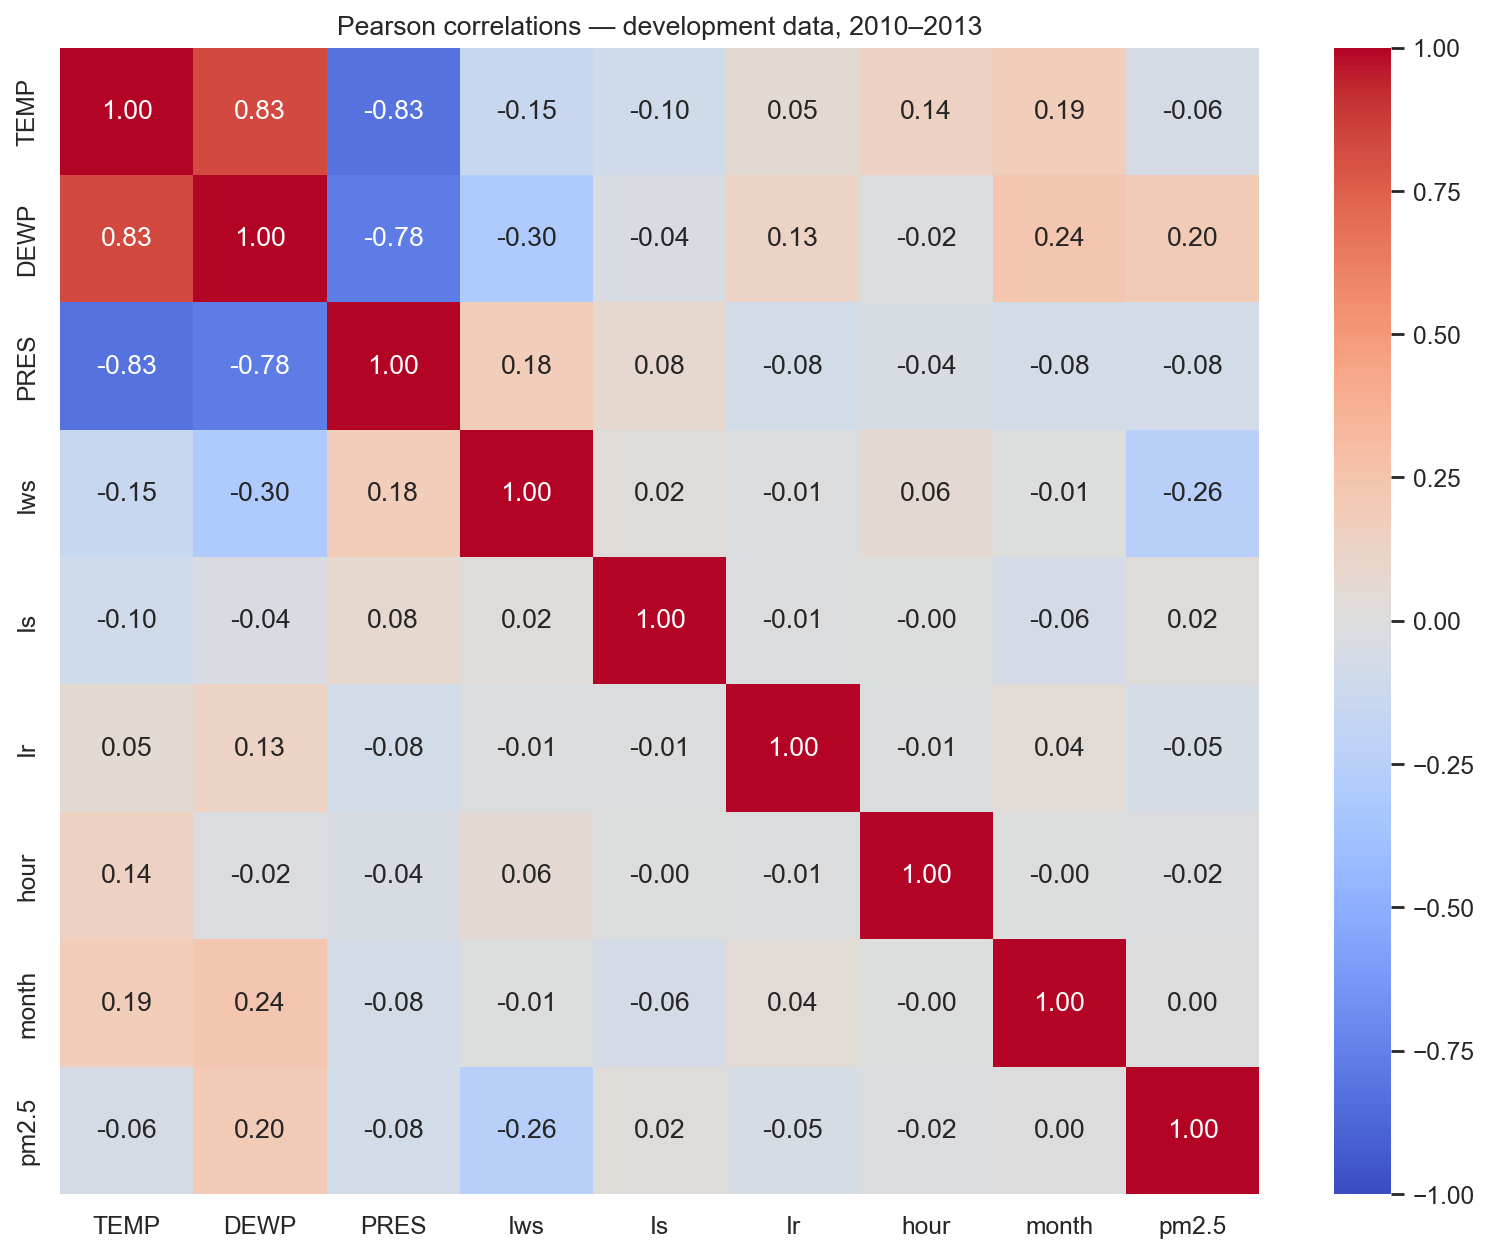
\includegraphics[width=0.82\textwidth]{figures/correlation_heatmap.png}
\caption{Pearson correlations among numeric inputs and PM2.5 on the 2010--2013 development data. These are descriptive associations, not causal effects.}\label{fig:correlation}
\end{figure}

\section{Discussion}
The results support the proposed expectation that a nonlinear tree ensemble can outperform simple linear regression on this historical dataset. Random Forest improves error measures without requiring a manually specified linear relationship between each weather variable and PM2.5. The near-identical performance of Linear and Ridge Regression suggests that the selected Ridge penalty did not meaningfully change predictive performance in this setup.

However, the best test $R^2$ of 0.417 indicates that substantial variation in hourly PM2.5 remains unexplained. The RMSE of 71.397 $\mu$g/m$^3$ is materially larger than the MAE of 48.073 $\mu$g/m$^3$, consistent with some relatively large errors. The actual-versus-predicted plots permit visual inspection of such errors, but the current experiment does not separately calculate error rates for extreme pollution episodes. Therefore, the original hypothesis that severe spikes would be underestimated has not been quantitatively established by this analysis.

Several limitations affect interpretation. First, weather observations are contemporaneous with the PM2.5 measurements, so these results do not establish next-hour or next-day forecasting performance. Second, the inputs omit direct measurements of emissions, traffic, and other possible drivers of air pollution. Third, this is one historical city and one held-out year; the results should not be assumed to transfer unchanged to present-day Beijing or other locations. Fourth, no systematic hyperparameter tuning, repeated time-series backtesting, uncertainty estimates, or formal feature-importance analysis was performed. Finally, dropping missing targets may introduce selection effects if the missing observations are not random.

Future work could define a one-hour-ahead target, restrict predictors to values known at forecast time, compare against a persistence baseline, use rolling chronological validation, and report performance specifically for high-PM2.5 episodes. These are suggestions, not experiments performed in the current project.

\section{Conclusion}
We compared four regression approaches for estimating hourly Beijing PM2.5 concentrations from weather and calendar features using a chronological train/validation/test design. On the held-out 2014 data, Random Forest performed best, achieving MAE 48.073 $\mu$g/m$^3$, RMSE 71.397 $\mu$g/m$^3$, and $R^2=0.417$. Linear Regression and Ridge Regression improved over the mean baseline but were less accurate than Random Forest. The study demonstrates the value of comparing a simple baseline with linear and nonlinear methods while keeping future-year observations separate for evaluation. Its conclusions concern historical same-hour estimation; a genuine future-hour forecasting system would require a different target and information-availability design.

\bibliographystyle{plainnat}
\begin{thebibliography}{9}
\bibitem[UCI Machine Learning Repository(2016)]{uci381} UCI Machine Learning Repository. \emph{Beijing PM2.5 Data}. Dataset 381. \url{https://archive.ics.uci.edu/dataset/381/beijing+pm2+5+data}. Accessed October 2026.
\bibitem[scikit-learn developers(2026a)]{sklearnlinear} scikit-learn developers. \emph{LinearRegression documentation}. \url{https://scikit-learn.org/stable/modules/generated/sklearn.linear_model.LinearRegression.html}.
\bibitem[scikit-learn developers(2026b)]{sklearnridge} scikit-learn developers. \emph{Ridge documentation}. \url{https://scikit-learn.org/stable/modules/generated/sklearn.linear_model.Ridge.html}.
\bibitem[scikit-learn developers(2026c)]{sklearnforest} scikit-learn developers. \emph{RandomForestRegressor documentation}. \url{https://scikit-learn.org/stable/modules/generated/sklearn.ensemble.RandomForestRegressor.html}.
\end{thebibliography}
\end{document}